\documentclass{report}
\usepackage[utf8]{inputenc}
\usepackage{fullpage}
\usepackage{graphicx}
\usepackage{booktabs}
\usepackage{color}
\usepackage{fancyhdr}
\usepackage{color}
\usepackage{colortbl}
\usepackage{amsmath,amssymb}
\usepackage{multido}
\usepackage{caption}
\usepackage{listings}

\lstnewenvironment{myc}
{\lstset{language=c}
\lstset{basicstyle=\footnotesize\ttfamily}
\lstset{keywordstyle=\color[rgb]{0,0,1}\bfseries}
\lstset{identifierstyle=\color{black}}
\lstset{commentstyle=\color[rgb]{0,0.4,0}}
\lstset{stringstyle=\color[rgb]{0.7,0,0}}
\lstset{showstringspaces=false}
\lstset{showtabs=false}
\lstset{tabsize=3}
\lstset{extendedchars=true}
\lstset{breaklines=true}
\lstset{postbreak={}}
\lstset{breakautoindent=true}
\lstset{breakindent=0pt}
\lstset{xleftmargin=0.1cm}
\lstset{xrightmargin=0cm}
\lstset{frame=tb,rulecolor=\color[gray]{.4}}
\lstset{captionpos=b}
\lstset{aboveskip=0.5cm,belowskip=0.5cm}
\lstset{numbers=left}
\lstset{columns=fixed}}
  {}
\title{LINGI2146 - Project - Attacks against RPL}
\author{Nicolas Houtain \& Nicolas Gorby Kabasele \& Arthur Paquot}
\renewcommand{\thesection}{\arabic{section}}

\begin{document}
\maketitle
\section{Introduction}
We choose as our subject for this project the attacks against the RPL
protocol. Nowadays, the internet of things gains more and more interest
and RPL could be one of the protocols used for those low power and lossy
networks. We were interested to see if this protocol is robust enough to
avoid an attack corrupting the network. In order to do so, we selected a
few known attacks for those kind of networks and we tried to implement
them in Contiki and simulate the behavior of the network with Cooja. The
different attacks that we present are a sinkhole attack, a
select-forwarding attack, a version number attack and a DAG
inconsistency attack. For each attack we briefly present the attack, how
we implemented it and how the network and the RPL protocol react to
those attacks with some measurement and countermeasure if any. For all
the attacks, the malicious behavior can be activated by pressing the
button of the mote. By pressing the button once, the node launches the
sinkhole attack, twice the version number attack, three times the select
forwarding attack and four times the DAG inconsistency attack. We only
changed the files contained in the folder contiki/core/net/rpl.

\section{Sinkhole attack}
A sinkhole attack is when a node announces an artificial beneficial
routing path. The other nodes of the network will therefore chose the
malicious node as their parent and most of the traffic will pass by the
malicious node.


\subsection*{Implementation}
We choose to implement the sinkhole attack by making the malicious node
announcing a rank higher that its real one. The malicious node will
advertise the rank 256 which the rank of the root. This is done in the
\textit{rpl-icmp6.c} in the method \textit{dio\_output}.


\begin{myc}
if(malicious){
	printf("The sinkhole attack is launched\n");
	dag->rank=(unsigned int) 256;
}
\end{myc}

\subsection*{Consequences on the network}
All the down neighbors of the malicious node chose it as their parent
since they think it's the root of the graph. A lot of the traffic will
therefore pass by the malicious node. This attack is powerful when
coupled with other attacks. Indeed, since an important part of the
traffic will pass by the malicious node, it has the opportunity to
corrupt, drop or do any other malicious action on the packets.



\subsection*{Measurement}
\begin{table}[h!]
	\centering
	\caption{Impact of  sinkhole on DAO MSG}
	\begin{tabular}{cccc}
		\toprule
		Type&DIO MSG & DAO MSG&time\\
		\midrule
		Non-malicious&31&1&2:30\\
		Malicious&31&25&2:30\\
		Non-malicious&35&1&3:45\\% A VERIFIER
		Malicious&35&30&3:45\\
		\bottomrule
	\end{tabular}
\end{table}
We can see that when the node advertises its fake rank, the number of
DAO messages it receives is significantly bigger. It receives 25 times
more packet in less than three minutes. We put different printf every
time the node receives a message and when the node chooses its parent.
We can see than once the attack is launched all the neighbors choose the
malicious node as parent. 

\section{Select-Forwarding Attack}
A select forwarding attack is an attack where a malicious node decides
arbitrarily which packet it will forward and which packet it will drop.
This kind of attack is really hard to detect for a protocol such as RPL
since the RPL packets are still distributed in the network, but all the
IPV6 packet for example, are dropped. The node that doesn't receive the
packet can not notice there is a bad behavior and the nodes that sent it
can think the packets were lost. 


\subsection*{Implementation}
We choose to drop all the IPV6 packets that the malicious node received
(packet that are not RPL packet). In order to do so, every time the
malicious node receives a ping packet, it will consider that its header
is wrong and will drop the packet. This is done in the
\textit{rpl-ext-header.c} file in the method
\textit{rpl\_verify\_header}, where the node, if malicious, returns "-1"
when verifying the header.  
\begin{myc}
if(malicious==3){
	printf("Malicious node drops the packet\n");
	return -1;
}	
\end{myc}

\subsection*{Consequences on the network}
When the malicious node is activated, all the ping packets that have to
reach a node to which the path pass by the malicious node are dropped.
This kind of attack is really powerful if coupled with a sinkhole
attack. In such case, most of the ping packets pass by the malicious
node and are discarded. 

\subsection*{Countermeasures}
It is difficult for a network to notify that some packet are lost,
especially with a protocol such as RPL where the lost of packet happens
really often. We let our little network running for several minute to
let RPL the time to spot the error, but no changes happened.

\subsection*{Measurement }
When the malicious behavior is not activated, every mote on the network
can be pinged from the outside thanks to the \textit{ping6} command.
However, when the mote becomes malicious, all the mote to which the path
pass by the malicious node are not pingable anymore. We put a printf in
the code to show when the malicious node drops the packets.\\ 
Note that this attack only works when using an IPV6 border router.

\section{Version Number Attack}
In the RPL protocol, each DIO message has a version number that is
incremented by the root each time a rebuilding of the DODAG is needed.
If a node has a version number smaller than the one of the root, it
means that the node has not migrated to the new DODAG and can therefore
not be used as a parent. If a malicious node increases the version
number of the DIO messages it sends, the other nodes will think that are
not up to date and will rebuild the DODAG graph and will reset their
timer.

\subsection*{Implementation}
In order to perform that attack, the malicious node, every time it sends
a DIO message, will increase the version number by one. This is done in
the \textit{rpl-icmp6.c} file in the method \textit{dis\_output}.

\begin{myc}
if (malicious==2){
    printf("Malicious node changes dag version for dio output.) %d instead of %d \n.", dag->version+1,dag->version);
	buffer[pos++] = dag->version+1;
} else {
	buffer[pos++] = dag->version;
}
\end{myc}

\subsection*{Consequences on the network}
This attack has several consequences on the behavior of the network. It
can create loop in the network, leading to the lost of packets and all
the successive and unnecessary rebuilding of the graph increase the
traffic of packets in the network. This consume the availability of the
links and the nodes that could be used for relevant traffic. This
overhead can exhaust the resources of the node and lead to a congestion
of the network. 
%[PARLER DES TIMER]

Moreover, the different nodes surrounding the malicious one will chose
it as their parent, since it has the most accurate version of the DODAG.
Finally, the malicious node will become the most used node of the
network, most of the messages passing by it. One minute after the
insertion of the first modified packet, the malicious node is the most
used node reaching after NOMBRE MINUTE the RADIO POURCENTAGE. 

\subsection*{Countermeasure}
A countermeasure for this attack could be a way to authenticate the
version number, i.e., that it was modified by the root and not by an
other node. With hash or cryptography mechanism, the version number of
the DIO packet could be verified by a node, if the hash value doesn't
correspond to the one expected, the version number is not taken into
account. Note that such a verification system will consume more
resources on the root, that has to use some mechanism to produce the
version number and on the different nodes that have to check the
correctness of the version number.

\subsection*{Measurement }
The consequence of the attack can be watched using the MPS stack viewer
provided by Cooja. We can observe that the stack of the nodes
surrounding the malicious one is much bigger when the attack has been
launched. Indeed, the reset of the different timers increases the
traffic of messages between the different nodes.\\


\begin{figure}
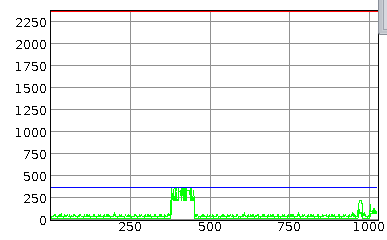
\includegraphics[scale=0.4]{img/normal_stack2}
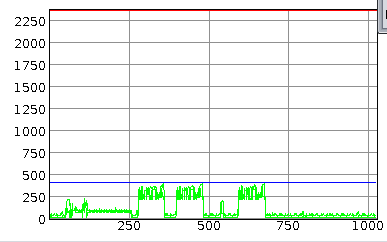
\includegraphics[scale=0.4]{img/normal_stack4}
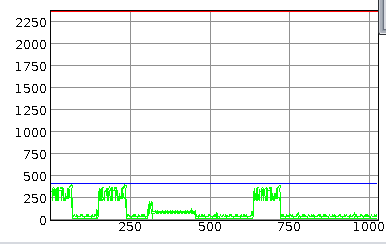
\includegraphics[scale=0.4]{img/normal_stack5}\\
\caption{Stack of a non-malicious node with no malicious node in the network}
\end{figure}

\begin{figure}
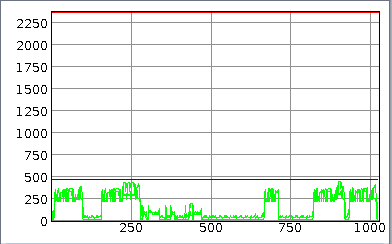
\includegraphics[scale=0.4]{img/mali_sta2}
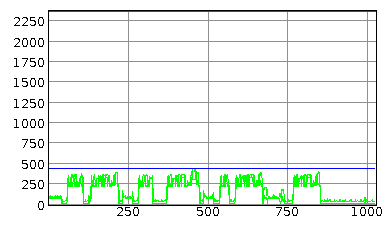
\includegraphics[scale=0.4]{img/mali_sta7}
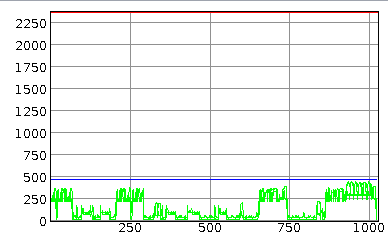
\includegraphics[scale=0.4]{img/mali_sta5}
\caption{Stack of a non-malicious with malicious node in the network}
\end{figure}

When the malicious node performs its attack, the stacks of the
non-malicious nodes surrounding it are almost never still. On the other
hand, when no malicious node is in the network, the stack can be still
for several seconds, grows when some messages are exchanged and then
becomes still again.\\

Moreover, we put a printf in the code to show when an inconsistency is
found, this leads to the reset of the timer, responsible of the increase
of teh traffic. The root also receives an DAG message with an
inconsistent version and it reset its timer too, to rebuild the DODAG.\\

We also analyzed the evolution of the traffic and the consumption of
resources by using the power tracker tool provided by Cooja. We first
let the network without malicious node in order to reach a stable state,
then after 4 minutes, we launched the attack. Immediately after the
attack is performed, the neighboring node chose the malicious one as
their parent and the power tracker show an increase of all the traffic
in the network. Indeed, the average of radio transmission and the node
with the highest rate increase over the time. The different results are
presented in the table below : in red, the traffic of the most used node
with a malicious node in the network, in green the average traffic with
a malicious node in the network and finally in blue, the average traffic
with no malicious node in the network. We can also see the evolution of
the ratio between the average traffic and the traffic of the most used
node. One minute after the insertion of the first corrupted packet, the
malicious node becomes the most used node and is responsible of most of
the traffic since the other node chose it as parent. 


% Simu avec les 14 noeuds : Apres 2min30, l'average est a 1,5 et le most used est à 2%, apres 3 min on est a 1,3 (average) et 1,7 (most used), après 4 min on est a 1,2 et 1,5. Apres 4 min le premier paquet corrupted est dans le réseau, 4min20
% A packet with the modified version is sent every 7 seconds approximatively 
%\begin{table}[h!]
%	\centering
%	\caption{Impact of  version number attack with Power tracker}
%	\begin{tabular}{ccccc}
%		\toprule"
%		Network attacked&Average traffic & Most used node&Ratio &time\\
%		\midrule
%		No & 1.50 \% &2.00 \%&1.33&2:30\\
%		No & 1.30 \% & 1.70 \% & 1.30& 3:00\\ 
%		No & 1.20 \% & 1.50 \% & 1.25&4:00\\
%		Yes & 1.50 \% & 2.20 \% & 1.46 & 4:20\\
%		Yes & 1.70 \% & 2.45 \% & 1.44 &4:30 \\
%		Yes & 1.88 \% & 2.60 \% & 1.38 & 4:40\\
%		Yes & 2.05 \% & 2.80 \% & 1.36 &4:50\\
%		Yes & 2.18 \% & 3.00 \% & 1.37& 5:00 \\
%		Yes & 2.30 \%& 3.37 \% & 1.46 & 5:10\\
%		Yes & 2.45 \% & 3.42 \% & 1.40 & 5:20 \\
%		Yes & 2.53 \% & 3.60 \% &1.42 &5:30\\
%		Yes & 2.80 \% & 3.98 \% & 1.42 &6:00\\
%		Yes & 2.88 \% & 4.19 \% & 1.45 & 6:10 \\
%		Yes & 3:08 \% & 4.65 \% & 1.51 & 6:40\\
%		Yes & 3.18 \%& 4.84 \%& 1.52 & 7:00\\	
%		Yes & 3.40 \% & 5.45 \% & 1.6 & 7:40 \\
%		Yes & 3.46 \% & 5.55 \% &  1.6 & 8:00 \\
%		\bottomrule
%	\end{tabular}
%\end{table}

\begin{figure}
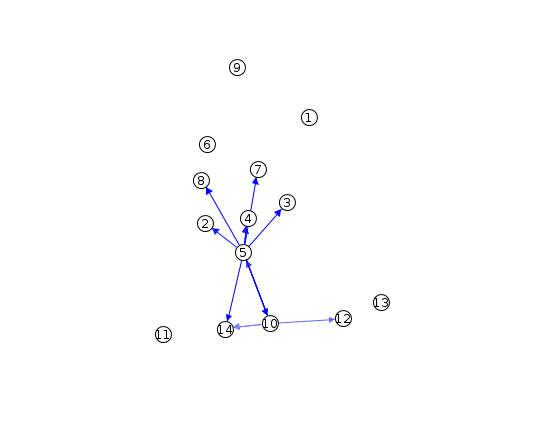
\includegraphics[scale=0.4]{img/versionStat2}
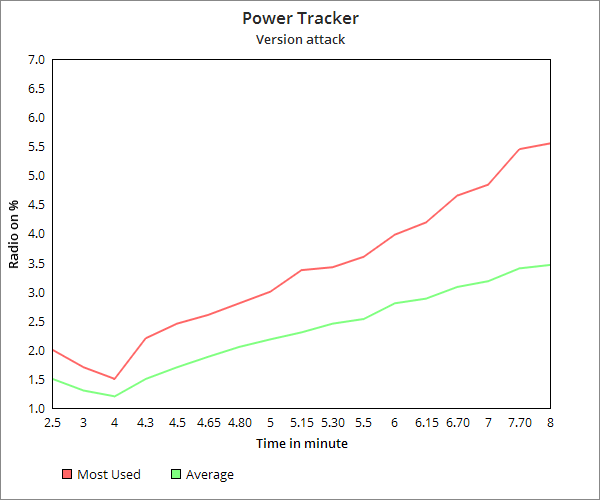
\includegraphics[scale=0.4]{img/versionStat}
\caption{Topology used : the malicious node is the mote 2 and the evolution of the radio traffic during a version number attack}
%\caption{}
\end{figure}


We used a built-in apps in contiki called \textbf{Powertrace} and \textbf{Energest} to measure the cpu 
consumption. This apps only provided an estimation but we can see that it is coherent with the
consequence we describded earlier. Each server mote print out the resource it currently used 
every 5 seconds. We run the simulation for 5 minutes. We launched the attack at 3 minutes.
Therefore we have 65 values for each server mote. To use Powertrace, we needed to remove
some code because the program was too big for the Z1 motes. We were only able to run it
on the normal mote, not the root one and the malicious one. 

As we can see on the figure below, the mote 7 is in the range of the malicious node and the mote
6 is not. We can see the attack as an impact on the two nodes but, the impact is less important
on the mote 6.


\begin{figure}[ht!]
\centering
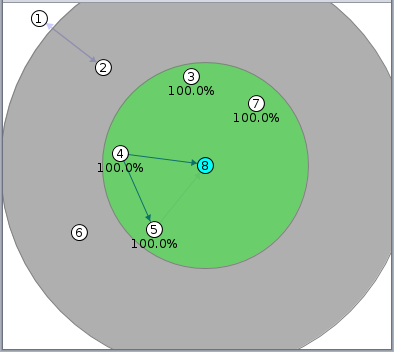
\includegraphics[scale=0.55]{img/simulation_measurement}
\caption{Topology:Mote 1 is the root and the malicious mote is the 8}
\end{figure}


%TODO Améliorer le graphe avec les .txt
\begin{figure}[ht!]
\centering
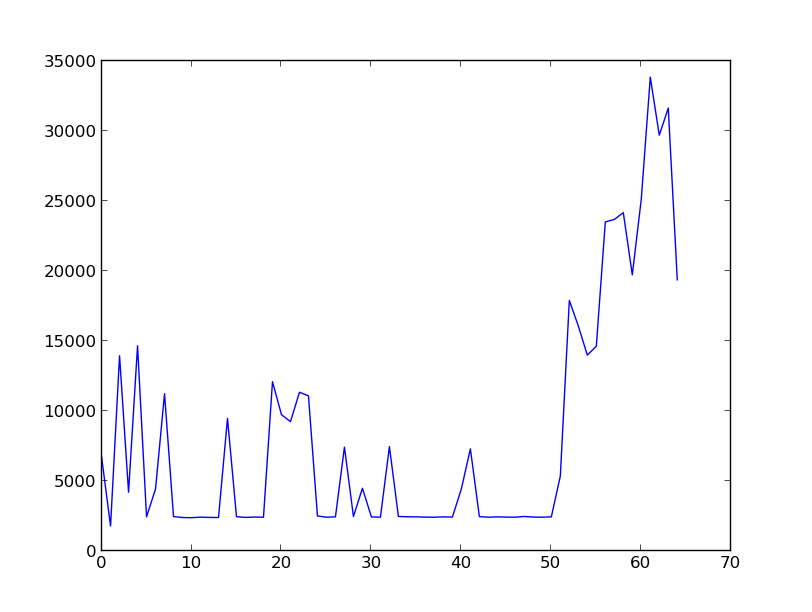
\includegraphics[scale=0.35]{img/mote6}
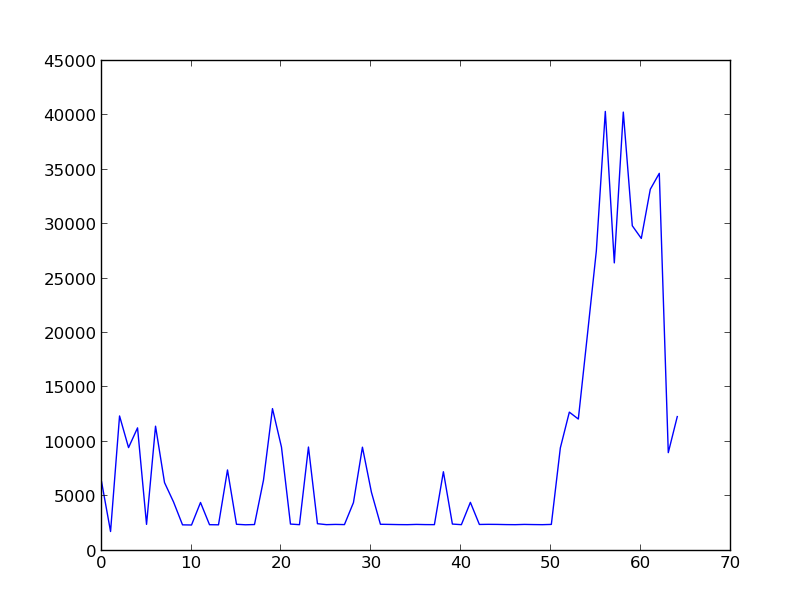
\includegraphics[scale=0.35]{img/mote7}
\caption{left: mote6, right:mote7}
\end{figure}



%http://www.chartgo.com/get.do?id=671333ad2b#.VziH_ddvfE8


\section{DAG Inconsistency Attack}
A DAG inconsistency is when the packet doesn't follow the direction that
matches the rank relationship. In that case, the node that notices the
inconsistency, it uses the rank error bit flag to advertise that this
packet is inconsistent. When a node receives an inconsistent packet with
the rank error bit set, it reset the timer and drop the packet. A
malicious node could therefore set the rank error bit of all the packet
it receives, leading to the reset of the timer and the lost of packet.\\

Note that the opposite attack is also possible, the malicious node
doesn't set the flag where a loop is detected. This attack is more
difficult to implement since we have to create loop in the network to
verify if the attack works, we therefore chose to implement the first
version.

\subsection*{Implementation}
The RPL protocol implemented in Contiki doesn't drop the packet when the rank error bit is set. However, it could be some situations where we would prefer to drop a packet that is inconsistent, we therefore changed the behavior of the RPL protocol to make it drop a packet when the rank error bit is set. The malicious node set the flag for all the packet it receives. This is done in the \textit{ext-header.c} file in the method [NAME].

\begin{myc}
if(malicious==4){
	printf("Malicious node changes the flag of the packet \n");
	UIP_EXT_HDR_OPT_RPL_BUF->flags |= RPL_HDR_OPT_RANK_ERR;
}

\end{myc}
\subsection*{Consequences on the network}
One of the immediate outcome of the attack is to reset the timer of the
node that receives the packet. The node will therefore send DIO message
more frequently, leading to an unnecessary used of the links and the
battery. The different neighbor of the node are also victim of the
attack since they have to process a useless traffic. Moreover, the node
will drop the different packet it receives with the flag set.

\subsection*{Countermeasures}

One solution could be to limit the number of time a node can reset its timer during a lapse of time. 


\subsection*{Measurement}
The DAG inconsistency results in the lost of packets and the reset of
the timers. The traffic is therefore increased. The printf in the code
shows when the loop or the inconsistency is discovered by a node,
resetting its timer and dropping the packet. When trying to ping a node
with the malicious node on the path, the packet will be discarded and
the ping will not work. 

\section{Other implementation}
In \textit{rpl.c}, when the button is pressed the method is called to
change the value of \textit{malicious} which represent the number of the
attack.

\begin{myc}
int malicious=0;
void
set_malicious(void){
	malicious = (malicious+1)%5;
}
\end{myc}

\end{document}
